% ---- pg-360 （书页 348） ----

\begin{mvfigure}
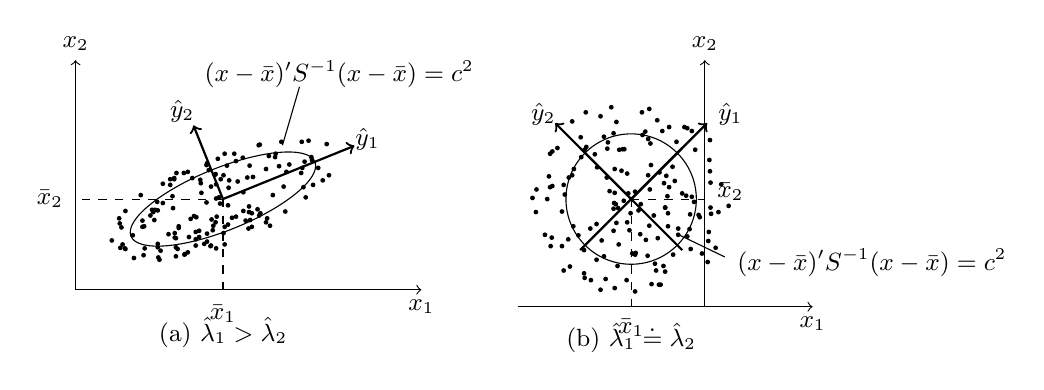
\begin{tikzpicture}[scale=0.72]
% ===== 图 (a) =====
\begin{scope}
\foreach \x/\y in {-0.48/-0.58, -1.12/-1.07, -0.48/-0.82, 0.63/0.95, -0.22/-0.83, 0.09/-0.45, 0.36/-0.21, -0.78/-0.51, 0.20/0.80, 1.46/0.03, 0.92/0.74, 0.03/-0.49, -0.40/0.34, 1.76/0.33, -1.23/-0.23, 0.46/-0.13, 0.47/0.59, -1.16/-0.05, 1.38/0.46, 0.16/-0.33, -1.82/-0.43, 0.61/-0.18, -1.73/-0.87, -0.11/-0.31, -0.47/-0.32, -0.28/-0.61, -0.17/-0.47, -1.06/-0.07, -1.83/-0.34, -0.29/-0.06, -0.12/0.26, -0.05/-0.08, -0.39/0.28, -0.88/-0.16, 0.64/-0.29, -1.72/-0.88, -1.10/-0.91, 1.44/0.66, -1.42/-0.38, -0.42/-0.56, -1.96/-0.73, 0.23/0.67, 1.42/0.21, 1.57/0.69, -0.60/-0.67, 0.78/-0.34, -0.62/0.48, 1.40/0.55, 0.35/0.73, -0.62/-0.94, -1.38/-0.87, 1.51/1.03, 0.76/0.53, -1.79/-0.50, -0.93/0.35, -0.09/0.71, -1.20/-0.19, 1.12/0.48, -0.21/-0.82, 0.83/-0.47, -1.40/-0.99, -0.07/0.03, -0.25/0.51, -0.80/-0.88, -0.48/-0.71, -0.83/-1.01, -0.20/-0.36, -0.78/-0.48, -0.42/-0.67, -0.93/0.25, -0.89/0.05, -0.14/0.43, 0.93/0.80, 1.68/0.55, -1.77/-0.80, 0.51/-0.25, -1.39/-0.48, 1.03/1.01, -0.12/0.01, -0.85/-0.68, 0.53/0.39, 0.43/0.38, 0.45/-0.52, -0.18/-0.55, 0.07/0.59, 1.07/0.22, 1.39/1.01, -1.45/0.07, 0.01/0.42, -1.57/-1.04, -0.29/0.60, -0.86/0.37, -0.54/0.37, 0.01/-0.60, -0.33/-0.79, -0.21/0.22, 0.09/-0.11, 0.81/0.76, -1.21/-0.37, -0.28/-0.75, -0.96/-0.62, -1.28/-0.29, -0.85/-0.60, 1.87/0.42, -0.83/-0.69, 0.88/0.07, 1.17/0.61, -1.72/-0.21, 0.36/0.12, -1.15/-0.20, 0.65/0.96, -0.82/0.46, -0.12/-0.87, 0.48/-0.37, -0.67/-0.97, -0.86/0.35, -1.15/-0.85, -0.51/-0.30, 1.59/0.25, 1.56/0.74, -0.69/0.46, 0.03/-0.80, -1.81/-0.86, 0.11/0.33, 0.03/0.80, 0.46/-0.23, -1.06/0.27, 0.51/-0.49, -0.13/-0.41, 1.10/-0.22, 0.23/-0.31, 0.26/0.31, -0.13/0.44, -1.42/-0.49, 0.99/0.58, -1.14/-1.03, 0.10/0.20, -0.28/0.63, -1.59/-0.64, -0.57/-0.35, 0.66/-0.25, -0.83/-0.85, -0.38/0.11, -1.15/-0.79, 0.40/-0.38, 1.83/0.97, 0.76/-0.41, -0.04/0.35, -0.68/-0.98, -1.25/-0.19}
  {\fill (\x,\y) circle (1.2pt);}
\draw[rotate=22] (0,0) ellipse [x radius=1.75, y radius=0.55];
\draw[->] (-2.6,-1.6) -- (-2.6,2.45) node[above,font=\small] {$x_2$};
\draw[->] (-2.6,-1.6) -- (3.5,-1.6) node[below,font=\small] {$x_1$};
\draw[dashed] (0,0) -- (0,-1.6);
\draw[dashed] (0,0) -- (-2.6,0);
\node[below,font=\small] at (0.0,-1.7) {$\bar{x}_1$};
\node[left,font=\small] at (-2.65,0) {$\bar{x}_2$};
\draw[->,thick] (0,0) -- (2.32,0.94);
\node[font=\small] at (2.55,1.05) {$\hat{y}_1$};
\draw[->,thick] (0,0) -- (-0.52,1.30);
\node[font=\small] at (-0.72,1.55) {$\hat{y}_2$};
\draw (1.35,1.98) -- (1.05,0.95);
\node[font=\small] at (2.05,2.2) {$(x-\bar{x})'S^{-1}(x-\bar{x})=c^2$};
\node[font=\small] at (0,-2.35) {(a) $\hat{\lambda}_1>\hat{\lambda}_2$};
\end{scope}
% ===== 图 (b) =====
\begin{scope}[shift={(7.2,0)}]
\foreach \x/\y in {1.41/-0.26, -1.43/0.21, -1.22/-0.22, -0.45/-1.41, -0.21/0.87, 0.67/0.21, 0.74/-0.98, -0.05/0.10, 1.39/1.04, 0.44/-1.26, 1.54/-0.23, -0.29/-1.57, 1.40/-0.15, -0.31/-0.56, 0.29/-1.00, -0.61/-1.07, 0.99/-0.66, 1.40/0.29, 0.50/0.47, 1.11/-0.05, -0.38/0.14, 1.03/-0.53, -1.19/-1.26, 0.36/-1.50, -0.60/0.56, -0.07/-0.41, 1.59/0.26, -1.39/0.84, -0.52/-0.73, 0.30/0.42, -1.11/-0.71, -0.26/-0.42, -0.15/0.88, 0.62/0.41, 0.73/0.57, 0.32/-0.47, -1.67/0.17, 1.39/0.49, -0.48/-1.01, 0.64/0.05, 0.46/1.39, 0.60/-1.28, 0.25/1.19, 0.19/1.53, 0.90/0.10, -0.41/1.00, -1.01/0.53, 0.33/0.17, 0.40/-0.29, -1.68/-0.23, 0.26/-0.72, 0.77/0.32, 1.36/-0.74, -1.04/1.37, -0.17/0.50, -0.89/1.09, -1.17/0.08, -1.39/0.23, -0.30/-0.07, -1.52/-0.63, 0.07/-1.63, -0.79/0.92, 0.80/1.01, -0.48/1.10, 0.42/-1.14, -1.30/0.90, 1.19/-0.28, -0.88/0.74, 0.57/-1.18, 1.49/-0.86, 0.60/-0.15, -1.22/-0.83, -0.31/1.16, 1.07/1.20, -0.07/0.45, 0.99/1.25, 0.07/0.13, 0.02/-0.96, 0.65/-0.48, 1.04/-0.27, 0.20/1.13, 0.30/1.06, -0.24/-1.18, -0.08/-1.43, -0.54/-1.60, 0.07/-0.98, -0.03/-0.55, -0.72/-0.52, -0.29/0.11, 1.21/-0.32, 0.49/-1.51, -1.45/0.40, -0.31/-0.17, 0.65/-0.25, 1.07/0.04, -0.43/0.38, -0.82/0.87, -1.40/-0.68, -0.13/-0.03, 0.13/-0.20, -0.23/-0.16, -0.64/0.79, 0.58/0.28, -0.80/1.53, -1.42/-0.83, -1.43/0.80, 1.38/0.69, -1.10/0.38, -0.54/1.46, 0.83/-0.52, -0.61/-0.44, -0.83/-0.90, -0.27/-0.09, -0.42/0.89, 0.47/-0.69, 0.55/1.20, 0.52/-1.51, -1.08/-1.19, 0.94/1.27, 1.13/0.87, 0.16/-0.62, -1.02/-0.48, 1.05/-0.88, 0.32/1.59, -0.35/1.62, -0.82/-1.39, -0.01/-0.25, 1.35/-1.11, 0.08/-0.95, 0.35/0.60, 0.34/0.98, 0.83/-0.63, -0.22/-0.80, -0.26/1.36, -0.93/-0.64, -1.04/0.42, -0.12/0.88, 1.37/-0.58, -0.29/0.53, -0.71/-1.43, -1.48/0.00, 0.97/0.06, -1.74/0.02, 1.25/-0.96, 0.67/1.27, -1.19/0.25, 1.72/-0.12, 0.17/-0.09, 0.60/-0.15, -0.83/-1.31}
  {\fill (\x,\y) circle (1.2pt);}
\draw (0,0) circle [radius=1.15];
\draw[->] (1.3,-1.9) -- (1.3,2.45) node[above,font=\small] {$x_2$};
\draw[->] (-2.0,-1.9) -- (3.2,-1.9) node[below,font=\small] {$x_1$};
\draw[dashed] (0,0) -- (1.3,0);
\draw[dashed] (0,0) -- (0,-1.9);
\node[below,font=\small] at (0,-1.95) {$\bar{x}_1$};
\node[right,font=\small] at (1.35,0.12) {$\bar{x}_2$};
\draw[thick] (-0.9,-0.9) -- (0.9,0.9);
\draw[->,thick] (0,0) -- (1.34,1.34);
\node[font=\small] at (1.75,1.5) {$\hat{y}_1$};
\draw[thick] (0.9,-0.9) -- (-0.9,0.9);
\draw[->,thick] (0,0) -- (-1.34,1.34);
\node[font=\small] at (-1.55,1.5) {$\hat{y}_2$};
\draw (1.65,-1.02) -- (0.82,-0.62);
\node[font=\small,anchor=west] at (1.7,-1.12) {$(x-\bar{x})'S^{-1}(x-\bar{x})=c^2$};
\node[font=\small] at (0,-2.45) {(b) $\hat{\lambda}_1\doteq\hat{\lambda}_2$};
\end{scope}
\end{tikzpicture}
\phantomsection\label{fig:8.4}\mvcap{图 8.4\quad 样本主成分和常数密度椭圆}
\end{mvfigure}

最后, 在直接对均值中心化数据 $\mathbf{x}_j-\bar{\mathbf{x}}$ 作近似时, 补充 8A 对样本主成分所起的作用给出了进一步结论.

\mvsub{样本主成分的标准化}

一般说来, 样本主成分在尺度改变时是不变的(练习 8.2). 正如我们在总体成分处理中提到的, 在不同尺度或在同一尺度但变化范围极其不同时所测量的变量, 常常要标准化. 例如, 利用下述构造完成标准化:
\phantomsection\label{eq:8-25}
\begin{equation}
\mathbf{z}_j=\mathbf{D}^{-1/2}(\mathbf{x}_j-\bar{\mathbf{x}})=
\begin{bmatrix}
\dfrac{x_{j1}-\bar{x}_1}{\sqrt{s_{11}}}\\[6pt]
\dfrac{x_{j2}-\bar{x}_2}{\sqrt{s_{22}}}\\[6pt]
\vdots\\[4pt]
\dfrac{x_{jp}-\bar{x}_p}{\sqrt{s_{pp}}}
\end{bmatrix}
\qquad j=1,2,\cdots,n \tag{8-25}
\end{equation}
将观测值标准化后的 $n\times p$ 数据矩阵
\phantomsection\label{eq:8-26}
\begin{equation}
\begin{aligned}
\mathbf{Z}&=\begin{bmatrix}\mathbf{z}_1'\\\mathbf{z}_2'\\\vdots\\\mathbf{z}_n'\end{bmatrix}
=\begin{bmatrix}z_{11}&z_{12}&\cdots&z_{1p}\\
z_{21}&z_{22}&\cdots&z_{2p}\\
\vdots&\vdots&&\vdots\\
z_{n1}&z_{n2}&\cdots&z_{np}\end{bmatrix}\\
&=\begin{bmatrix}
\dfrac{x_{11}-\bar{x}_1}{\sqrt{s_{11}}}&\dfrac{x_{12}-\bar{x}_2}{\sqrt{s_{22}}}&\cdots&\dfrac{x_{1p}-\bar{x}_p}{\sqrt{s_{pp}}}\\[8pt]
\dfrac{x_{21}-\bar{x}_1}{\sqrt{s_{11}}}&\dfrac{x_{22}-\bar{x}_2}{\sqrt{s_{22}}}&\cdots&\dfrac{x_{2p}-\bar{x}_p}{\sqrt{s_{pp}}}\\[8pt]
\vdots&\vdots&&\vdots\\[4pt]
\dfrac{x_{n1}-\bar{x}_1}{\sqrt{s_{11}}}&\dfrac{x_{n2}-\bar{x}_2}{\sqrt{s_{22}}}&\cdots&\dfrac{x_{np}-\bar{x}_p}{\sqrt{s_{pp}}}
\end{bmatrix}
\end{aligned}
\tag{8-26}
\end{equation}
产生样本均值向量[见\hyperref[eq:3-27]{式(3-27)}]
